\chapter{Orbits}

\textit{Without proper experiments I conclude nothing.}\\
\noindent\textbf{-   Johannes Kepler}

\begin{marginfigure}%
  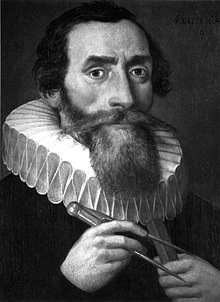
\includegraphics[width=\linewidth]{kepler.jpg}
  \caption{This 1610 portrait shows Kepler, at age 39, with his chopsticks.}
  \label{fig:marginfig}
\end{marginfigure}

\section{History}
Johannes Kepler was a German mathematician, astronomer, and astrologer. A key figure in the 17th century scientific revolution, he is best known for his laws of planetary motion.  His work advanced the Copernican heliocentric model.  From 1600 to 1610 Kepler took over the observational work of Tycho Brahe, publishing star charts in 1627, known as the \textit{Rudolphine Tables}.  In this time Kepler collaborated with Galileo and advanced fundamental optics through development of the refracting telescope.  Kepler provided foundations for Isaac Newton's theory of universal gravitation.

\begin{marginfigure}[100pt]
  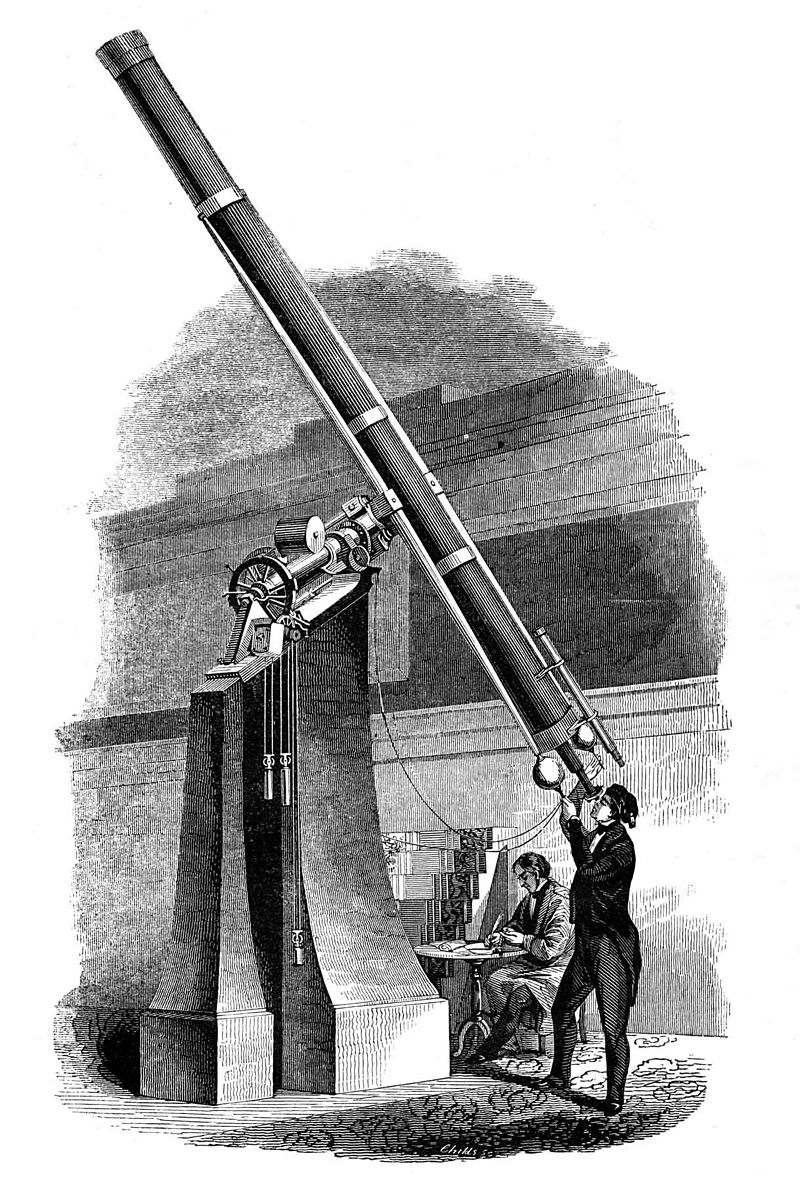
\includegraphics[width=\linewidth]{telescope.jpg}
  \caption{Refracting telescope from the Cincinnati Observatory in 1848.}
  \label{fig:marginfig}
\end{marginfigure}

\section{Kepler's Laws}
Kepler's Laws are three statements describing the motion of planets around the sun.

\begin{enumerate}
\item The orbit of a planet is an ellipse with the Sun at one of the two foci.
\item A line segment joining a planet and the Sun sweeps out equal areas during equal intervals of time.
\item The square of the orbital period of a planet is proportional to the cube of the semi-major axis of its orbit.
\end{enumerate}


\newpage

\section{Circular Orbital Motion}
\vspace{0.5cm}

\subsection{General}

\begin{marginfigure}
\begin{tikzpicture}[scale=0.55]	
\draw [color=gray!80] (0,0)--(3,0) node [midway,anchor=south,inner sep=1pt, outer sep=1pt]{$r$};


\begin{scope}[shift={(0,0)}, scale=1,rotate=120] 
 	\draw[color=gray,dashed] (0,0) circle (3cm);
	
	\begin{scope}[shift={(0,-4)}, scale=0.75, rotate=-90] 
		\draw[ thick,-stealth] (0,-0.1) -- (0,0.8) node [near start,anchor=east]{\scriptsize $\theta$};  
		\draw[thick](-0.1,0) -- (0.1,0);
		\draw[thick](0.2,-0.4) -- (0.2,-0.6);
		\draw[ thick,-stealth] (0.1,-0.5) -- (1,-0.5) node [near start,anchor=north]{\scriptsize $r$};  
	\end{scope}
	
	\fill[black] (0,0) circle (1mm);  
	\fill[color=white] (0.5,-2.5) -- (-0.5,-2.5) -- (-0.5,-3.5) -- (0.5,-3.5) -- cycle;
	\draw[very thick] (0,-3) circle (0.5cm);
 	\draw (0,-3) node {$m$};
 \end{scope}	
 	  
 \begin{scope}[shift={(7,0)}, scale=1,rotate=120] 
 	\draw[->,thick] (0,0) -- (0,1.3) node [anchor=east ,scale=1] {$F_{c}$}; 	 
    	\fill[black] (0,0) circle (0.5mm);   
\end{scope}

\end{tikzpicture}
  \caption{General circular orbit}
  \label{fig:fig}
\end{marginfigure}

The speed in circular orbit is the product of radius and angular velocity.
$$v=\omega r$$
There is some force causing centripetal acceleration.   
$$\overrightarrow{F}_c=-\frac{mv^2}{r}\hat{r}=-m\omega^2r\hat{r}$$
The kinetic energy turns out to be half the product of this force and the radius of orbit.
$$KE=\frac{mv^2}{2}=\frac{F_cr}{2}$$
%$$-\nabla PE= \overrightarrow{F}_c$$





\subsection{Gravity}
For planetary orbits gravity is the force causing centripetal acceleration.  
$$\overrightarrow{F}_c=-\frac{mMG}{r^2}\hat{r}$$
Using Newton's law of universal gravitation, the potential energy is identified.
$$PE=-\frac{mMG}{r}$$
For an circular motion from an inverse square force law, such as that for gravity or electrostatics, the kinetic energy is half the negative potential energy and the total energy is negative and equal in magnitude to the kinetic energy.
 
$$KE=\frac{F_cr}{2}=\frac{mMG}{2r}=-\frac{PE}{2}$$
$$E=-KE$$
\subsubsection{Period of Gravitational Orbit}
\begin{marginfigure}[0pt]
  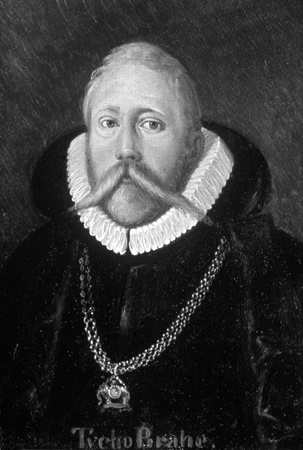
\includegraphics[width=\linewidth]{brahe.jpg}
  \caption{Tycho Brahe was a slick dutchman with a sweet 'stache and a brass nose.}
  \label{fig:marginfig}
\end{marginfigure}
Kepler's third law is easily derived for circular gravitational orbits by equating the centripetal force and the universal gravitational force.
$$m\omega^2r=\frac{mMG}{r^2}$$
This can be used to express the relationship between the period and radius of orbit.
$$T=\frac{2\pi}{\omega}=\sqrt{\frac{4\pi^2 r^3}{MG}}$$


\newpage

\begin{marginfigure}[0pt]
  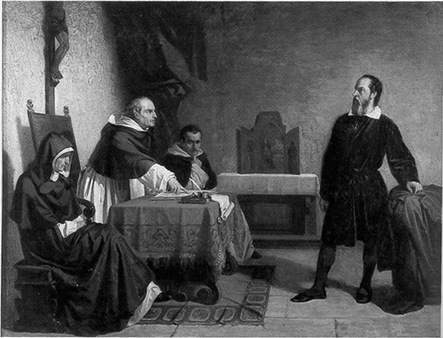
\includegraphics[width=\linewidth]{galileo.jpg}
  
  \caption{Cristiano Banti's 1857 painting \textit{Galileo facing the Roman Inquisition}.}
  \label{fig:marginfig}
\end{marginfigure}
\subsection{Central Spring}
The following represents the situation when the force causing centripetal acceleration is Hookean.  
$$\overrightarrow{F}_c=-kr\hat{r}$$
In this case the potential energy and kinetic energy are equal.
$$PE=\frac{kr^2}{2}$$
$$KE=\frac{F_cr}{2}=\frac{kr^2}{2}=PE$$
$$E=2KE$$
\marginnote{The Hookean centripetal force is of interest because it arises in the case of gravitational attraction to a sphere of uniformly distributed mass.}
\subsubsection{Period of Spring Orbit}
The angular velocity and period of orbit are derived as follows.
$$m\omega^2r=kr$$
$$\omega=\sqrt{\frac{k}{m}}$$
$$T=\frac{2\pi}{\omega}$$


\section{Elliptic Gravitational Orbits}
\subsection{Kepler's First Law}
The orbit of every planet is an ellipse with the Sun at one of the two foci.
\subsubsection{Conservation Laws}
$$E=KE+PE=\frac{mv^2}{2}-\frac{mMG}{r}=\text{constant}$$
$$L=mr^2\omega=\text{constant}$$
\marginnote{A conic section is a curve obtained as the intersection of a cone with a plane.  The eccentricity, e, determines if the conic section is a hyperbola, parabola, ellipse or a circle.  e =  0 the section is a circle.  0<e<1 the section is an ellipse.  e=1, a parabola and e>1 a hyperbola.}
\subsubsection{Conic Sections and Eccentricity}
$$r=\frac{r_0}{1+e\cos{\theta}}$$
$$e^2=1+\frac{2Er_0}{GMm}$$
\vspace{1cm}

\subsection{Kepler's Second Law}
A line joining a planet and the Sun sweeps out equal areas during equal intervals of time.\\ \ \\

In an infinitesimally small length of time, $\Delta t$, the line joining the sun and planet sweeps out an infinitesimally small area, $\Delta A$.
$$\frac{\Delta A}{\Delta t}=\frac{1}{2}r v_{tan}=\frac{1}{2}r^2\omega$$
The rate of change of the swept out area is directly proportional to the angular momentum.
$$\frac{\Delta A}{\Delta t}=\frac{L}{2}$$
Since the angular momentum is constant so is the rate of change of the area.
$$\frac{\Delta A}{\Delta t}=\text{constant}$$

\begin{figure}
$$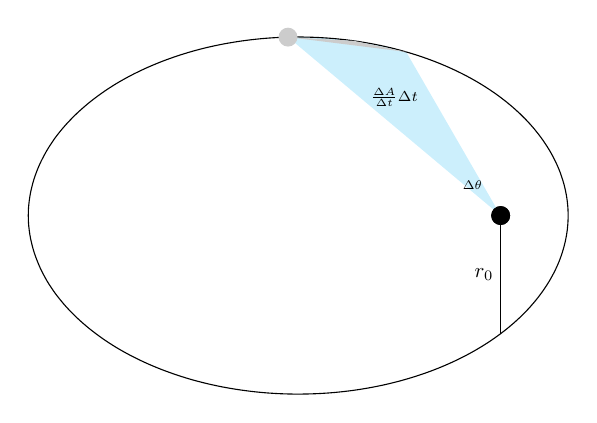
\begin{tikzpicture}
    [line cap=round,line join=round,x=2cm,y=2cm, scale=1.5, decoration={brace,amplitude=2pt}]
%main layer
%creating the ticks and xy-axis nodes
%some function
\fill[fill=cyan!20] (0,0) -- plot [samples=200,domain=120:140] ({0.5*cos(\x)/(1+0.75*cos(\x))},{0.5*sin(\x)/(1+0.75*cos(\x)}) -- cycle;

 \draw[smooth,samples=200,domain=0:360]
                                 plot({0.5*cos(\x)/(1+0.75*cos(\x))},{0.5*sin(\x)/(1+0.75*cos(\x)});
 
\fill[fill=black!20] plot [samples=3,domain=120:140] ({0.5*cos(\x)/(1+0.75*cos(\x))},{0.5*sin(\x)/(1+0.75*cos(\x)}) circle (0.8mm);


    \fill[black] (0,0) circle (0.8mm) node [anchor=north ,scale=1] {$ $};
     \fill[black] (0,0) circle (0.8mm) node [anchor=north ,scale=1] {$ $};
     %\fill[black] (1.75,0) circle (0.3mm) node [anchor=north ,scale=1] {$t_f$};
      %  \fill[black] (0,0.25) circle (0.3mm) node [anchor=south east,scale=1] {\scriptsize$ v(0)$};

  %\draw[-latex,color=black,thin] (-0.2,0) -- (2,0) node [anchor=north ,scale=1] {$t$};
   %\draw[-latex,color=black,thin] (0,-0.2) -- (0,1.4)node [anchor=east ,scale=1] {$F$};
    \draw (0,0) -- (0,-0.5) node [midway, anchor=east ,scale=0.75] {$r_0$};
      \draw (-0.45,0.5) node [anchor=center,scale=0.75] {\scriptsize $\frac{\Delta A}{\Delta t}\Delta t$};
       \draw (-0.12,0.13) node [anchor=center,scale=0.65] {\scriptsize $\Delta \theta$};
       % \draw (1,0.35) node [anchor=center ,scale=1] {$\Delta p$};
         %\draw[<->,color=black,thin] (0.25,-0.2) -- (1.75,-0.2)node [midway,anchor=south ,scale=1] {$\Delta t$};
        
 \end{tikzpicture}$$
  \caption{Kepler's third law is an outcome of conservation of angular momentum.}
  \label{fig:fig}
\end{figure}

